\newpage\section{Design and Development of the Artefacts}

The artifact, which is intended to improve experimental research in behavioral research in data analytics, is to be implemented as a software component or application. In this step, a suitable architecture is developed based on the established requirements. For this purpose, the application is first fundamentally conceptualized. This involves analyzing possible technologies and the corresponding processes. The architecture is then implemented in practice on the basis of this basic conceptualization.

\subsection{Process Conceptualization}\label{subsec:ProcessConcept}

%This section focuses on the basic design of the application. For this purpose, the processes based on the requirements are presented first, which must be implemented by the application. Subsequently, technologies are presented which are used for their implementation.

%\subsubsection{Process Mechanisms}

In order to effectively implement the requirements for the application, the processes described by the requirements and validated by the test cases are represented in the following swim lane diagrams. The goal of this is to illustrate the individual processes in a technology-independent manner. The reason for this is that the individual processes are initially presented in generalized form, irrespective of technological restrictions or limitations. The following Swim Lane diagrams represent the individual steps of the experiment. Swim lane diagrams depict processes by showing business activities in relation to each other and how they are associated with each other (\cite{Caudle.2009}).A large part of the final functionalities can be divided into two different categories. An example of this are the requirements (F2, F3 and N5.1), whereby the application should offer both the possibility to read in and save user data and data corresponding to the experiment setup itself. These requirements can be summarized in functions and data concerning the experiment and functions and data concerning the participants. The two lanes \enquote{Participant Repository} and \enquote{Experiment Repository} are representative for those two categories and data sources. The \enquote{User} lane shows the activities performed by the test subjects, the \enquote{Experimental Repository} lane shows all activities that can be associated with the experimental setup, and the \enquote{Patricipant Repository} lane shows all data and activities that are related to the test subjects. 

\begin{figure}[htbp]
    \centering
    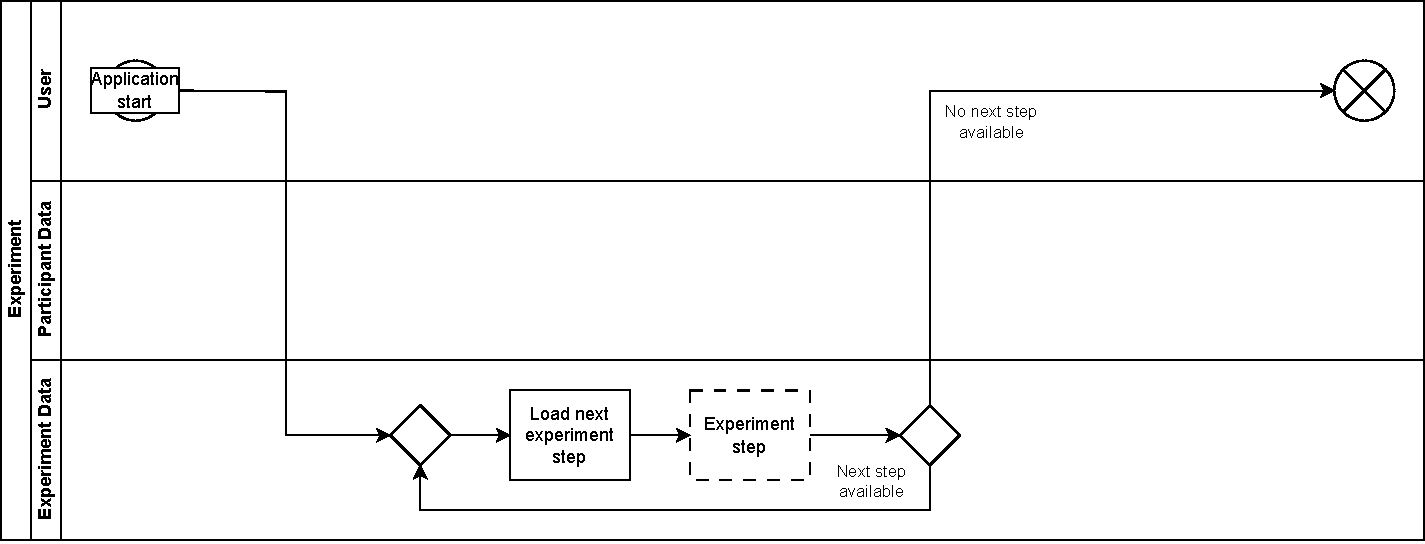
\includegraphics[width=0.99\textwidth, keepaspectratio]{content/05_design_and_dev_artefacts/ExperimentSwimLane.drawio.pdf}
    \caption{Experiment - Swim lane}    
    \label{fig:experimentSwimLane}
\end{figure}

Figure \ref{fig:experimentSwimLane} shows the basic structure of an experiment with the conceptualized application. The whole experiment is divided into different experiment steps, which are executed one after the other until the experiment is completed. The application is started first and then the first step of the experiment is executed. This could be for example an information message for the participants. After that the next step is executed if another step is available. If no further step is available, the experiment ends. This simple abstraction of an experiment concentrates on the essentials and thus allows the most flexible and adaptable construction kit for an experiment. The individual steps of the experiment, which are executed one after the other, can be customized by the person performing the experiment as well as mapped by standard steps. The standard steps represent steps which have to be used in a multitude of experiments and thus partially represent requirements. In the following, some of these experiment steps which illustrate standard steps that are included in the application are illustrated with the help of swim lane diagrams. Figure \ref{fig:DataInputSwimLane}, \ref{fig:groupAllocationSwimLane}, \ref{fig:questionairSwimLane} and \ref{fig:infoScreenSwimLane} represent these standard steps. The dashed box \enquote{Experimental Step} of figur \ref{fig:experimentSwimLane} can be replaced by any number of these. For this reason, the graphics mentioned also begin and end in the \enquote{Experimental Repository} lane.

\begin{figure}[htbp]
    \centering
    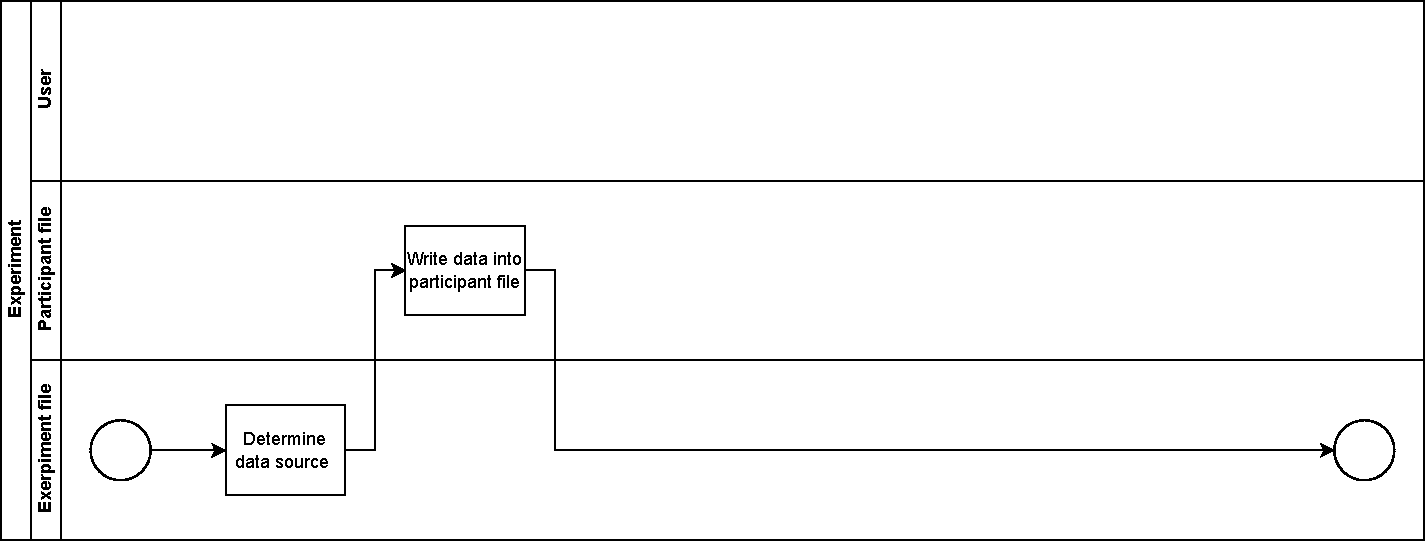
\includegraphics[width=0.99\textwidth, keepaspectratio]{content/05_design_and_dev_artefacts/DataInputSwimLane.drawio.pdf}
    \caption{Data input step - Swim lane}    
    \label{fig:DataInputSwimLane}
\end{figure}

Figure \ref{fig:DataInputSwimLane} represents the process step of reading data from one or more sources. The assumption is that this data must first be processed or standardized before it can be meaningfully assigned to the participants.

\begin{figure}[htbp]
    \centering
    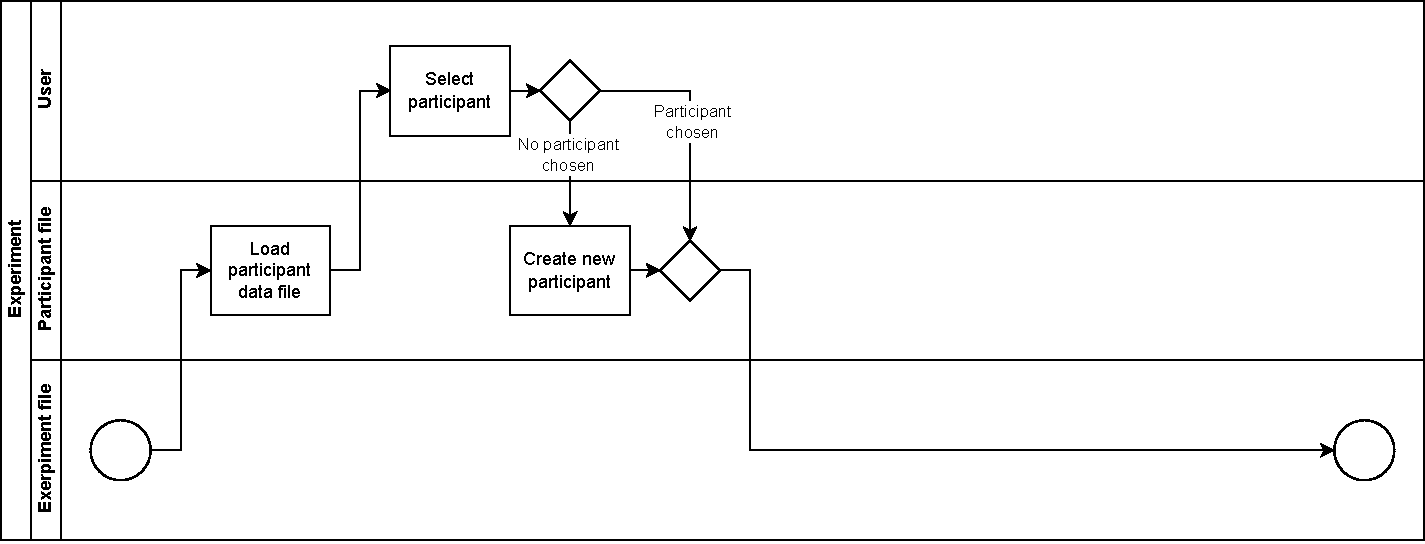
\includegraphics[width=0.99\textwidth, keepaspectratio]{content/05_design_and_dev_artefacts/ChooseTestSubjectSwimLane.drawio.pdf}
    \caption{Choose test subject step - Swim lane}    
    \label{fig:ChooseTestSubjectSwimLane}
\end{figure}

Figure \ref{fig:ChooseTestSubjectSwimLane} enables the mapping between the test subject and their ID which will be used for the rest of the experiment.

\begin{figure}[htbp]
    \centering
    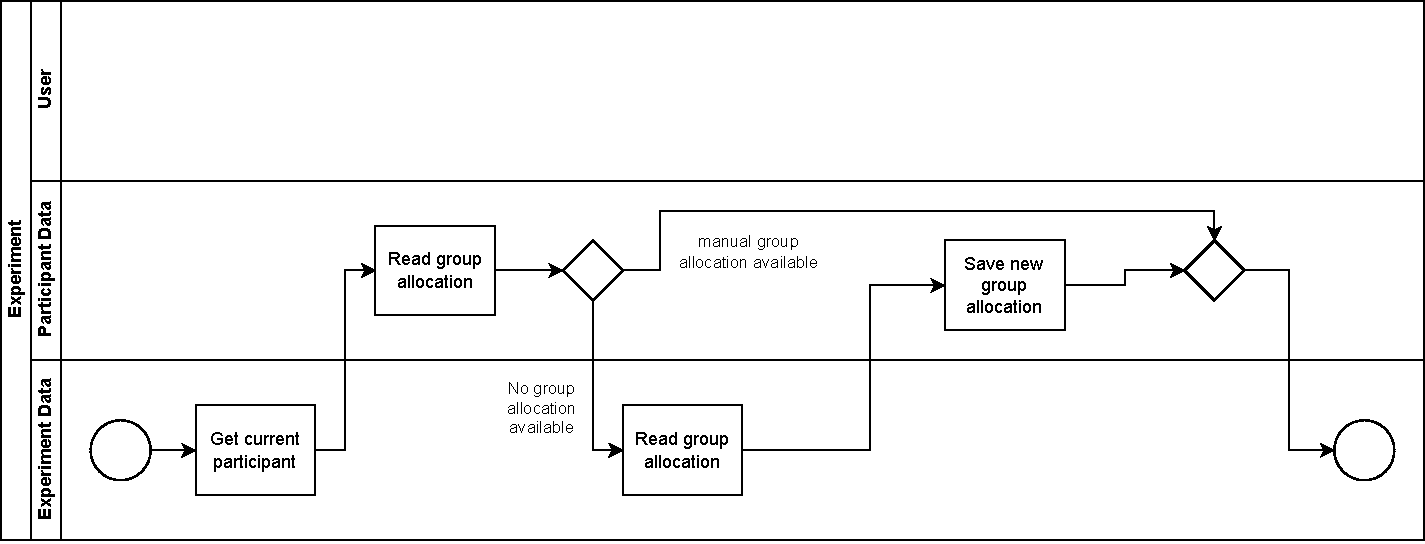
\includegraphics[width=0.99\textwidth, keepaspectratio]{content/05_design_and_dev_artefacts/GroupAllocationSwimLane.drawio.pdf}
    \caption{Group allocation step - Swim lane}    
    \label{fig:groupAllocationSwimLane}
\end{figure}

Figure \ref{fig:groupAllocationSwimLane} represents the process of assigning individual participants into groups. This can either be the case that participants are divided according to a predefined group, arbitrarily or according to certain criteria.

\begin{figure}[htbp]
    \centering
    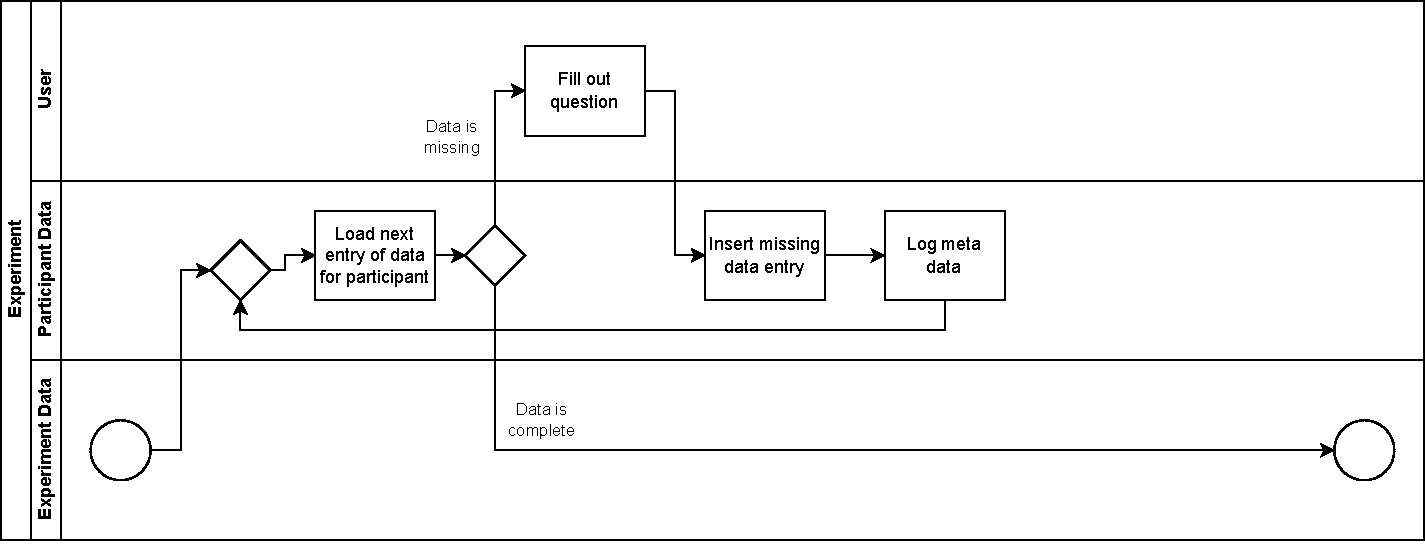
\includegraphics[width=0.99\textwidth, keepaspectratio]{content/05_design_and_dev_artefacts/QuestionairSwimLane.drawio.pdf}
    \caption{Questionair step - Swim lane}    
    \label{fig:questionairSwimLane}
\end{figure}

Figure \ref{fig:questionairSwimLane} is used to complete mising information or data about the participants. For this purpose, test subjects are asked questions based on missing data entries. This process is conceptualized similarly to the general experiment setup, so that any number of questions or no questions are displayed for completion, depending on the number of missing data points about a test subject. An example would be a test subject for which the age is missing. An input field is automatically displayed for the participant to fill in the missing data about himself. If all data for a test subject is complete, nothing is displayed.

\begin{figure}[htbp]
    \centering
    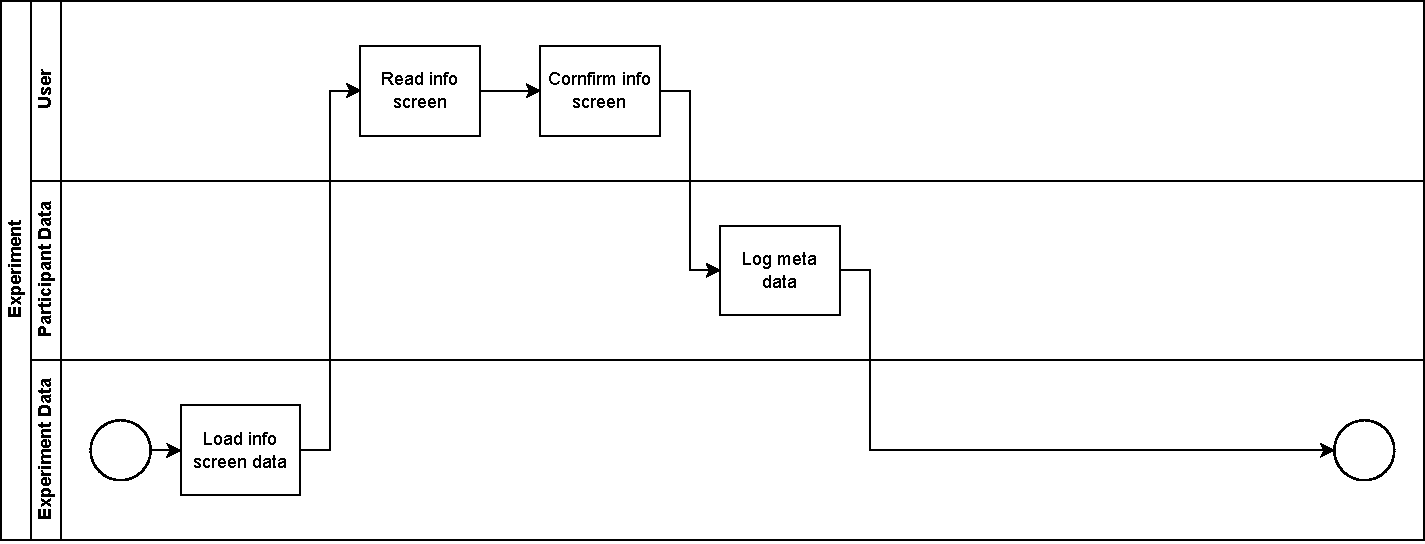
\includegraphics[width=0.99\textwidth, keepaspectratio]{content/05_design_and_dev_artefacts/InfoScreenSwimLane.drawio.pdf}
    \caption{Info screen step - Swim lane}    
    \label{fig:infoScreenSwimLane}
\end{figure}

Figure \ref{fig:infoScreenSwimLane} displays information to the test subjects and can be used both as a means of notification during an experiment and as a representation of information.

\subsection{Technology Selection}

In order to select appropriate technologies for the implementation of the application, the established requirements must be considered. It can be assumed that all functional requirements can be implemented by any modern programming language that is turing complete. The non-functional requirements N3.1 (Evaluation of Data), N3.2 (Vizualize Final Data), N7.1 (Multi-Source) are represented by the availability of various interfaces. Furthermore, the two non-functional requirements N1.2 (Time-Flexibility) and N6.1 (Monitoring of Study) are not relevant to the technology selection as these refer to the way the application is implemented and not its technological nature. This leaves requirements N1.1 (Distand Communication),  N4.1 (Simplicity), N5.1 (Reusable), N5.2 (Interoperability), N5.3 (Openness of Platform), N8.1 (Advanced User Interface) and the afformentioned availability of interfaces as requirements for selecting a suitable technology. In the following chapters, various technologies and tools are presented that are intended to meet these requirements.

%interfaces
%Distand Communication
%Simplicity
%Reusable
%Interoperability
%Openness of Platform
%Advanced User Interface


\subsubsection{Android and Android Studio}

Android is an open source operating system for mobile devices which was first announced by Google in 2013. To date, Android has achieved a market share of over 90\% in the mobile sector and is the most used operating system over all, being used in almost every second device (\cite{statcounter.2023}, \cite{Richter.2019}). The standard development environment to develop Android is the \ac{ide} Android Studio, which supports a wide range of developer tools and functionalities. As an open source project and, due to its high distribution on various devices Android suits the openness of platform and interoperability requirement (\cite{Richter.2019}). Applications for the Android operating system are called apps. These apps are programs designed for touch inputs, which are specifically designed for mobile devices. However, as a widely used open source operating system, Android also supports other input options, advanced network capabilities and a variety of interfaces and extensions (\cite{Richter.2019}). Thus it can be assumed that the interface and distand communication requirements can be fulfilled through the usage of Android. The two programming languages that can be used to develop these Android apps are Java and Kotlin. These apps then can be tested either directly on an Android device or on a variety of virtual devices integrated in Android Studio, which further facilitates the development of said applications (\cite{Richter.2019}). As a mobile operating system, one of Android's main focuses is the user interface as an input function, in addition to network functionalities and a variety of interfaces. Android therefore has a wide range of design guidelines, interface functionalities and is updated at very regular intervals (\cite{statista.2023}, \cite{Richter.2019}). Due to these regular updates, the widespread use of Android and the focus on \ac{ui} intensive use cases, it can be assumed that an app developed in Android supports the latest user interface technologies and therefore fulfills the advanced user interface requirement.


\subsubsection{Java}

Java is a programming language originally developed by Microsystems. Since 2009 Java is part of the product portfolio of Oracle Corporation. Java is an object-oriented programming language, which makes it an universally applicable and robust programming language (\cite{Ullenboom.2017}). Unlike many other programming languages, one of the special features of Java is its platform independence. Most programming languages use a compiler or interpreter to translate program code into byte code, which varies depending on the hardware and can only be executed on the appropriate processors. Java avoids this limitation by first having a compiler translate the Java program code into byte code, which is then executed via an interpreter in a virtual environment which is called \ac{jvm}. In this way, Java code can theoretically be executed on any system (\cite{Ullenboom.2017}). This makes Java not only a programming language but also a runtime system, which is made clear by the naming of the Java Platform by Oracle. The Java Platform supports beside Java itself also the execution of some other programming languages as for example Kotlin (\cite{kotlinlang.2023}). Due to this fact, Java is especially suitable for the implementation of the artefact based on the requirements N5.1 (Reusable) and N5.2 (Interoperability). Java also supports a variety of programming concepts through standard libraries. These include data structures, string processing, date/time processing, graphical interfaces, input/output, network operations, threads and more (\cite{Ullenboom.2017}), which ensures the N1.1 (Distand Communication) requirement and the availability of interfaces. The Java runtime environment also enables fast code execution and comes with various utilities such as a garbage collector and output name handlers. The syntax of Java is generally considered to be very easy to understand and beginner-friendly (\cite{Ullenboom.2017}), fulfilling the requirement N4.1 (Simplicity). In addition to technical aspects, Java is also Open-Source, extremely widespread, popular and a variety of literature for it is available (\cite{Ullenboom.2017}), which generally indicates an openness of platform (Requirement N5.3 Openness of Platform) and convenient to develope code (N4.1 (Simplicity)). Disadvantages of Java, which are also mentioned for the sake of completeness, mainly relate to very specific platform-dependent use cases. Since Java was developed as a general-purpose programming language and platform-independent, it is very difficult to access hardware or drivers directly. However, these use cases are irrelevant in the course of this work (\cite{Ullenboom.2017}). 


\subsection{System Architecture Development}

Overall, it can be summarized that the non-functional requirements, which consider properties of the system, are completely fulfilled by using the Android operating system in combination with the Java programming language. In general, most of the requirements could already be met by both Android and Java alone, so the combination of the two provides a solid foundation for meeting the remaining requirements. However, as already noted in Section \ref{subsec:reqSpec}, the fulfillment of the non-functional requirements is by no means a binary state, but can be partly of a subjective nature, which is why no test cases could be set up for these requirements. Taking the above arguments into account, and especially the extremely wide distribution of the Android operating system, the technical combination of Android and Java for the implementation of the artifact is considered the best option. Furthermore, there is the possibility that at a later point in time another technology combination may be able to better reflect the requirements. At this point in time, however, the requirements can best be met by the combination of Android and Java. In addition, for the reasons mentioned, it can be assumed that this combination of technologies will remain the best way to implement the requirements in the long term. However, the fact that these technologies will no longer be up to date at a later point in time exists, but cannot be ruled out for any other technology too. On the contrary, Android and Java are a sensible and sustainable choice in the long term for the above-mentioned reasons according to the current state of research. For this reason, the artifact is implemented in the form of a mobile Android application.

\begin{figure}[htbp]
    \centering
    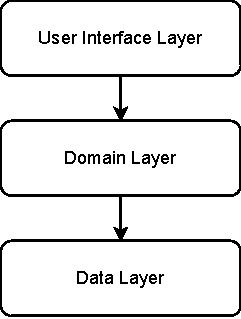
\includegraphics[width=0.33\textwidth, keepaspectratio]{content/05_design_and_dev_artefacts/ArchitectureBestPracticeAndroid.drawio.pdf}
    \caption[Android App Architecture]{Android App Architecture (\cite{Google.2023})}    
    \label{fig:androidAppArchitecture}
\end{figure}

The recommended architecture for an Android app is shown in Figure \ref{fig:androidAppArchitecture} and consists of three layers, the \ac{ui} layer, the domain layer, and the data layer. The \ac{ui} layer displays application data and the app itself to the user. The \ac{ui} layer is further divided into \enquote{\ac{ui} elements} and \enquote{State Holders}. \enquote{\ac{ui} elements} correspond to the displayed screen elements and the \enquote{State Holders} to temporary data of the current state of the \ac{ui}. The domain layer is optional. It is used for abstraction and structuring of the data layer and is recommended above all if the application is to represent very complex business cases or the application must be designed to be very reusable (\cite{Google.2023}). Due to the requirements N5.1 (Reusable), a domain layer is therefore used in the conceptualized application. Classes in this layer are usually called use cases or interactions and always represent a single functionality. For example, the output of the time could be a functionality that must be used by several components. This functionality would then be represented by a \textit{GetTime} class. The data layer contains the data and business logic of the application (\cite{Google.2023}). This layer defines to what extent data is processed, modified or stored. It is also divided into two parts, the repositories and the data sources (\cite{Google.2023}). The repositories are responsible for exposing the data to the rest of the application, to centralize changes to the data and to resolve conflicts between data sources. A repository can contain zero or multiple data sources. The repositories also contain the business logic and abstract the data sources from the rest of the application. Each data source is represented by one data source class which is the link between the system for data operations and the application. Sources for these data sources could be a file, a network or a local data base (\cite{Google.2023}). The communication between the individual layers is solved in Java via so-called call-back methods. Call-back methods are special methods to which program code is passed, which is executed at a certain time or event and which then notifies the higher-level program. In this way, the call-back function does not have to be modified each time, but said program code can be passed. An example would be a data retrieval, the code for this is passed using a call-back method, which is then executes when the event that the queue is processed is triggered, which then notifies the parent program of its execution and result (\cite{Zaccagnino.2020}). In the following, the concrete implementation of the architecture of the artifact is presented. The technical components are divided into the \ac{ui} layer, the domain layer and the data layer. 

\subsubsection{Data Layer}

The individual data sources are masked from the rest of the application by the so-called repositories. In principle, however, a large number of different data sources can be used. Among others, local files, database systems or network storage.  The number of data sources can vary between none and any number. The individual data sources depend on the respective experiment, which is implemented with the help of the artifact that is developed in this thesis. For this reason, a simple local CSV file is used as a placeholder for different data sources. This is done for the sake of simplicity, in the final application this placeholder file can then be replaced by any other sources. The important part of the design work is the repositories and how they process the data. The actual data sources are negligible and strongly dependent on the use case. The data layer as a whole corresponds to the \textit{Particpant Data} and \textit{Epxeriment Data} lanes from the previously defined processes \ref{fig:experimentSwimLane}, \ref{fig:DataInputSwimLane}, \ref{fig:ChooseTestSubjectSwimLane}, \ref{fig:groupAllocationSwimLane}, \ref{fig:questionairSwimLane} and \ref{fig:infoScreenSwimLane} as these contain the business logic for elements associated with the experiment itself and the test subjects respectively. For this reason and in order to clearly abstract the standard data sources of the artefact from potential data sources that get implemented within experiments two repositories called \textit{ParticipantRepository} and \textit{ExperimentRepository} are implemented. The ParticipantRepository could also contain multiple data sources for information about the participants. This architecture is illustrated in Figure \ref{fig:dataLayer}. As already mentioned, the conceptual design of the artifact is limited to a single data source for the experiment itself and the participants for the sake of simplicity. This is reflect by the colored elements of Figur \ref{fig:dataLayer}, the gray parts are only exemplary placeholders for an extension of the data sources.

\begin{figure}[htbp]
    \centering
    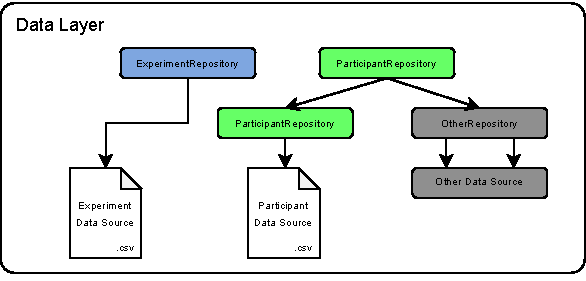
\includegraphics[width=0.79\textwidth, keepaspectratio]{content/05_design_and_dev_artefacts/DataLayer.drawio.pdf}
    \caption{Data Layer of the Artefact}    
    \label{fig:dataLayer}
\end{figure}

%Daten Layer entspricht den Swim Lanes Epxeriment and Patricipant weil hier die Business Logik liegt

\subsubsection{Domain Layer}

The domain layer is an optional layer that encapsulates complex business logic or logic that needs to be reused frequently (\cite{Google.2023}). Since it is not known to what extent the individual elements will be used in an experiment and a special focus is placed on the reusability of the individual components, this optional layer is implemented in the artifact. Further advantages resulting from the use of a domain layer are the avoidance of duplicated code, the improved readability of the architecture, an improvement in the testability of the app and the avoidance of large classes by splitting the tasks. The domain layer classes are accessed in the same way by the \ac{ui} as repositories of the data layer are accessed. An example of a domain layer class would be to request the addresses of the best authors of the year to send them an award. In this example there would be two data sources with repositories, one for authors and their addresses and another one containing the best selling books including authors. A domain layer class would hide access to these two repositories and the complex logic of determining the addresses of the best authors of the year from the rest of the application. To keep the classes of the domain layer simple it is adviced that each class should contain only a single functionality and should not contain mutable data (\cite{Google.2023}). These individual functions are also called use cases. Use cases (Domain Layer classes) can call each other and can be hierarchically dependent with each othre within the domain layer as needed. Since one use case is supposed to represent one function at a time, a domain layer class (or use case) is created for each function or action  that appears in one of the process swim lane diagrams in the \textit{Experiment Data} and \textit{Participant Data} lane from section \ref{subsec:ProcessConcept}. Since these UseCases can be layered arbitrarily in the domain layer, UseCases are also created for all processes that do not contain user interaction, i.e., Swin Lane diagram \ref{fig:groupAllocationSwimLane}.

%1 Determin Data Source
%2 Load Participant Data File: GetParticipantDataUseCase
%3 Create New Participant : CreateNewParticipantUseCase
%4 Read Group Allocation Participant : GetGroupAllocationPUseCase
%5 Read Group Allocation Experiment : GetGroupAllocationEUseCase
%6 Allocate Groups : AllocateGroupsUseCase
%7 Load next entry of data for participant : GetNextDataEntryUseCase
%8 Log meta data : LogMetaDataUseCase
%9 Load info screen data : GetInfoScreenDataUseCase


\subsubsection{User Interface Layer}

The concept of graphical user interfaces is implemented in Android via so-called activities. While the entry in regular Java applications takes place via a \textit{main()} method, an Android application initiates code via activities. The Android developer documentation describes an activity as \enquote{[...] entry point for an app's interaction with the user} (\cite{Google.2023}). The required \ac{ui} elements of the app are generated in the activity. An activity corresponds to a screen. Apps can contain several different UI screens and thus several different activities. Activities can also call other activities and navigate to them as desired. An app is therefore a sequence of different activities that represent different screens. Usually, an activity serves as the entry point to the app. This activty, also called the main activty, is the first screen that is shown when the application is started. Although Activities together form a complete app, Activities are only very superficially connected to each other. Basically, each activity is a replaceable, self-contained component that can be called in any order. This reusability and separation makes Activities the perfect foundation to implement the individual \enquote{experiment steps} described in Section \ref{subsec:ProcessConcept}. Based on this fact and the fact that an Activity corresponds to a \ac{ui}, a separate Activity is designed for each process step from Section \ref{subsec:ProcessConcept}. The three experiment steps, which include user inputs are the \textit{choose test subject}, \textit{questionair} and \textit{info screen} step, depicted in figure \ref{fig:ChooseTestSubjectSwimLane}, \ref{fig:questionairSwimLane} and \ref{fig:infoScreenSwimLane}. Figure \ref{fig:uiPrototypeArtefact} depicts these three use cases as a \ac{ui} prototype. Figure \ref{subfig:chooseTestSubject} represents the process step of choosing a test subject depicted in figure \ref{fig:ChooseTestSubjectSwimLane}. Figure \ref{subfig:Questionair} represents the process step of letting the test subject answer questions depicted in figure \ref{fig:questionairSwimLane}. Figure \ref{subfig:InfoScreen}  represents the process step of showing information to the test subject depicted in figure \ref{fig:infoScreenSwimLane}. The three \ac{ui} sketches show the basic division of \ac{ui} elements, to which the actual implementation of the activities is oriented. Furthermore, further custom steps from an experiment would also be implemented using Activities. In this way, the reusability and separation of the individual experiment steps is guaranteed.


\begin{figure}[htbp]
    \centering
    \begin{subfigure}[b]{0.3\textwidth}
        \centering
        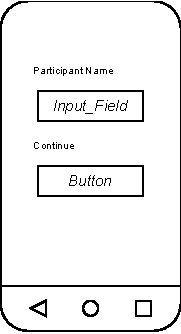
\includegraphics[width=\textwidth]{content/05_design_and_dev_artefacts/ActivityParticipantChoose.drawio.pdf}
        \caption{Choose test subject step}
        \label{subfig:chooseTestSubject}
    \end{subfigure}
    \hfill
    \begin{subfigure}[b]{0.3\textwidth}
        \centering
        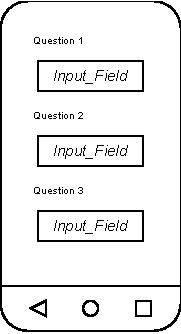
\includegraphics[width=\textwidth]{content/05_design_and_dev_artefacts/ActivityQuestionair.drawio.pdf}
        \caption{ Questionair step}
        \label{subfig:Questionair}
    \end{subfigure}
    \hfill
    \begin{subfigure}[b]{0.3\textwidth}
        \centering
        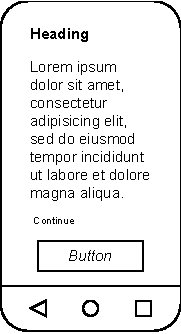
\includegraphics[width=\textwidth]{content/05_design_and_dev_artefacts/ActivityInfoScreen.drawio.pdf}
        \caption{Info screen step}
        \label{subfig:InfoScreen}
    \end{subfigure}
       \caption{User Interface Prototype of Artefact}
       \label{fig:uiPrototypeArtefact}
\end{figure}

After the basic UI has been designed, the navigation between the individual steps must be conceptualized and implemented. Generally, the sequence of screen calls is stored in the manifest of the application (\cite{Google.2023}).

\subsection{Consolidated System Architectural Summary}\label{subsec:completeArchitecture}

In general, it can be summarized that the processes that have been illustrated by swim lane diagrams have been technically implemented as follows:
\begin{itemize}
    \item Diagram A depicts the process of an experiment in general. The event "Experiment Step" is representative for all other Swim Lane process diagrams.
    \item The "User" lane of the diagrams represents the interaction of the user. The individual events in this lane are therefore represented by UI activities.
    \item For each diagram that does not contain a user input and is therefore not represented by an activity, a UseCase is also created.
    \item The lane "Experiment Data" and "Participant Data" are representative for all events which are associated with data of the respective parts. 
    \item The actual data resides in various data sources and is abstracted from the rest of the application by repositories. Although the two swim lanes are representative of the data layer, data source and repository are not illustrated into the swim lanes.
    \item The individual events of the "Experiment Data" and "Participant Data" lanes are each represented by a single use case and thus form the domain layer.
\end{itemize}

%Next step: Navigation behandeln

%Android Developer Doku (\cite{Google.2023})

%Grundsätzlich wird auf die Umsetzung der Navigation und Experimentreihenfolge durch Cucstomizing verzichtet, da Customizing die Komplexität einer Anwendung nicht verringert und die User Experience nicht verbessert im Gegensatz zur Umsetzung des Customizings durch Coding. Gleichzeitig Customizing aber extreme Einschränkungen mit sich bringt. ist blöd (\cite{Chou.2008})


%\begin{figure}[htbp]
%    \centering
%    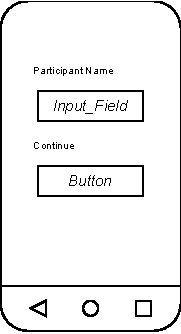
\includegraphics[width=0.4\textwidth, keepaspectratio]{content/05_design_and_dev_artefacts/ActivityParticipantChoose.drawio.pdf}
%    \caption{Adroid Studio Activitys}    
%    \label{fig:activitiesMockUp}
%\end{figure}



%\subsubsection{Customizing and System Output}

%This section is intended to provide an overview of the technological framework used and the basic architecture of the application. This section focuses primarily on a basic overview, while the next sections go into more detail about the individual components.




%\subsection{Prototype Development}
